% Created 2017-03-24 Fri 13:49
\documentclass[10pt,t,a4paper]{beamer}
\usepackage[utf8]{inputenc}
\usepackage[T1]{fontenc}
\usepackage{fixltx2e}
\usepackage{graphicx}
\usepackage{longtable}
\usepackage{float}
\usepackage{wrapfig}
\usepackage{rotating}
\usepackage[normalem]{ulem}
\usepackage{amsmath}
\usepackage{textcomp}
\usepackage{marvosym}
\usepackage{wasysym}
\usepackage{amssymb}
\usepackage{hyperref}
\tolerance=1000
\usetheme{BTH_msv}
\author{Mikael Svahnberg\thanks{Mikael.Svahnberg@bth.se}}
\date{2016-04-06}
\title{Design Patterns}
\hypersetup{
  pdfkeywords={},
  pdfsubject={},
  pdfcreator={Emacs 25.1.1 (Org mode 8.2.10)}}
\begin{document}

\maketitle

\section{Classroom}
\label{sec-1}
\begin{frame}[label=sec-1-1]{Responsibility-Driven Design}
Responsibility for \alert{Doing}
\begin{itemize}
\item Doing something (e.g. a calculation)
\item Creating other objects
\item Initiating an action in another object
\item Controlling and coordinating other objects
\end{itemize}

Responsibility for \alert{Knowing}
\begin{itemize}
\item Knowing about private encapsulated data
\item Knowing about related objects
\item Knowing about things it can derive or calculate
\end{itemize}
\end{frame}
\begin{frame}[label=sec-1-2]{Levels of Patterns}
Different levels:
\begin{itemize}
\item Architecture
\begin{itemize}
\item Systems, subsystems
\end{itemize}
\item Design
\begin{itemize}
\item Classes, groups of classes
\end{itemize}
\item Idioms
\begin{itemize}
\item One class, functions within one class
\end{itemize}
\item GRASP
\begin{itemize}
\item In some sense orthogonal
\item Learning aid for OO Design
\item Advice for Assigning Responsibilities
\end{itemize}
\end{itemize}
\end{frame}
\begin{frame}[label=sec-1-3]{GRASP Patterns}
(Listed on the inside of the book cover)
\begin{itemize}
\item Information Expert
\item Creator
\item Controller
\item Low Coupling
\item High Cohesion
\item Polymorphism
\item Pure Fabrication
\item Indirection
\item Protected Variations
\end{itemize}
\end{frame}
\begin{frame}[fragile,label=sec-1-4]{Example: GRASP Patterns}
 \vspace{-1cm}\hspace{2cm}
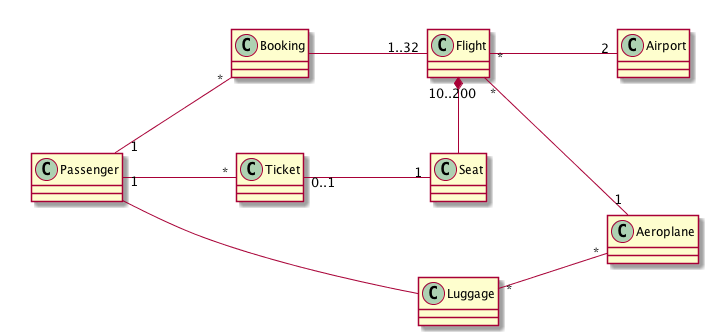
\includegraphics[height=4cm]{FGRASPExample.png}

\begin{block}{Discuss}
\begin{itemize}
\item Who should calculate the cost of a \texttt{Booking}?
\item Who should be responsible for creating a \texttt{Ticket}?
\item Why should a \texttt{Passenger} not be aware of the \texttt{Flight}?
\item How should a \texttt{Passenger} interact with this system when booking a trip?
\item How would you implement first, business, and third class?
\end{itemize}
\end{block}
\end{frame}

\begin{frame}[label=sec-1-5]{Example: Design Patterns in Pacman}
A look at the game:

\begin{itemize}
\item The game consists of scenes (Main Menu, Actual Game, High-Score List)
\item Each scene consists of a number of [different] objects (graphical as well as audio)
\item Some objects need awareness of other objects
\item Some objects in each scene needs to deal with UI input
\end{itemize}
\end{frame}

\begin{frame}[fragile,label=sec-1-6]{Different Scenes}
 \begin{itemize}
\item Problem: The game consists of several scenes (Main Menu, Actual Game, High-Score List)
\item Design Pattern: Strategy
\item Involved Classes: Context, \texttt{<<abstract>> Strategy}, ConcreteStrategy*
\item Pacman: Game, \texttt{<<abstract>> BasicScene}, MenuScene, GameScene
\end{itemize}

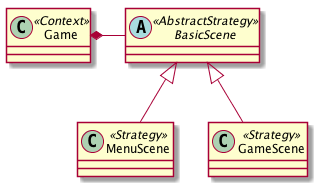
\includegraphics[height=4cm]{FPM_Scenes.png}
\end{frame}

\begin{frame}[fragile,label=sec-1-7]{Creating Objects for different Scenes}
 \begin{itemize}
\item Problem: Set up all objects necessary for each Scene
\item Design Pattern: Builder
\item Involved classes: Director, \texttt{<<abstract>> Builder}, ConcreteBuilder*
\item Pacman: MenuScene/GameScene, \texttt{<<abstract>> WorldCreator}, GameCreator, MenuCreator
\end{itemize}
\vspace{1cm}
\begin{itemize}
\item Design Pattern: Factory Method
\item Involved classes: Creator (with \texttt{<<abstract>>FactoryMethod()}), ConcreteCreator (with instantiated FactoryMethod())*
\item Pacman: Scene (with \texttt{<<abstract>>createObjects()}), GameCreator (with instantiated createObjects()), \ldots
\end{itemize}
\end{frame}
\begin{frame}[fragile,label=sec-1-8]{Behaviour of Ghosts I}
 \begin{itemize}
\item Problem: Each ghost behaves in a different way.
\item Design Pattern: Strategy
\item Involved Classes: Context, \texttt{<<abstract>> Strategy}, ConcreteStrategy*
\item Pacman: Ghost, \texttt{<<abstract>> GhostMovementStrategy}, BlinkyStrategy, InkyStrategy, PinkyStrategy, ClydeStrategy
\end{itemize}
\end{frame}
\begin{frame}[label=sec-1-9]{Only one Audio/Graphics/World}
\begin{itemize}
\item Problem: Avoid creating more than one instance of AudioManagement, GraphicsManagement, World
\item Design Pattern: Singleton
\item Involved Classes: Singleton (with static getInstance(), private constructor)
\item \alert{Less Optional Alternative:} Coding Pattern: Only create stuff in one place, keep central repository with pointers to these objects.
\end{itemize}
\end{frame}
\begin{frame}[label=sec-1-10]{Redirecting Input}
\begin{itemize}
\item Problem: Different objects are interested in UI input
\item Design Pattern: Observer
\item Involved Classes: Observable, Observer
\item Pacman: InputManager, PacmanObject, MainMenuObject
\end{itemize}
\end{frame}
\begin{frame}[fragile,label=sec-1-11]{Behaviour of Ghosts II}
 \begin{itemize}
\item Problem: When pacman eats supercandy, the behaviour of the ghosts change
\item Design Pattern: State
\item Involved Classes: Context, \texttt{<<abstract>> State}, ConcreteState*
\item Pacman: Ghost, \texttt{<<abstract>> GhostState}, GhostNormalState (see above, GhostStrategy), GhostChasedState
\end{itemize}
\end{frame}
\begin{frame}[label=sec-1-12]{Architecture Patterns}
Examples of Systems:

\begin{itemize}
\item Compiler
\item Interactive System, e.g. a Time Management Program
\end{itemize}

\only<2>{
$\ldots$ imposed with different quality requirements:
\begin{itemize}
\item Performance: High Throughput
\item Flexibility / Continuous Deployment
\end{itemize}
}
\end{frame}
\begin{frame}[label=sec-1-13]{Discuss: When to worry about Design Patterns}
When should you introduce patterns into your system?
\begin{itemize}
\item GRASP patterns
\item Design Patterns
\item Architectural Patterns
\end{itemize}
\end{frame}
% Emacs 25.1.1 (Org mode 8.2.10)
\end{document}